\section{Introduction}
\label{sec:intro}

Sparse Merkle Trees (SMTs) are Merkle trees over large logical address spaces. A height-$h$ SMT has $2^h$ possible leaf coordinates, but only a small subset of leaves is usually occupied. Empty subtrees are represented by publicly known default hashes. This default-hash mechanism makes SMTs a common building block for revocation maps, authenticated dictionaries, and blockchain state commitments~\cite{sparsemt,revtrans,jmt,ethereum,zcash}. Despite the sparse representation, membership verification keeps the standard Merkle proof interface: a verifier checks a leaf value together with one sibling digest per level and recomputes the committed root.

\textbf{Problem of interest.} The standard SMT proof API is efficient, but it reveals the queried target. When a client requests a membership proof, the server learns which key, account, certificate, or state object is being checked, and it also observes the corresponding authenticated path. Existing SMT work mainly improves storage, proof generation, multiproofs, and updates. These optimizations reduce the cost of proof serving, but they do not provide query privacy. This paper studies private retrieval of SMT membership proofs for a fixed public snapshot: the snapshot and its public metadata may be known, while the queried occupied leaf should remain hidden.

\textbf{Generic batch-PIR baseline.} Private information retrieval (PIR) is the natural tool for hiding a database index, but an SMT membership proof is not a single database record. A standard proof is a height-$h$ array of sibling digests. Some of these digests are non-default values that must be obtained from the server, while others are default hashes that the client can reconstruct locally from the public default-hash chain. Running one independent PIR query per proof level would hide the target, but it would treat a structured Merkle proof as $h$ unrelated private lookups.

Thus, private SMT proof retrieval is better viewed as a structured batch-PIR problem. The client must retrieve several sibling digests using a target-independent query pattern, without revealing which Merkle path those digests belong to. Generic batch-PIR techniques can privately retrieve multiple records, but they treat the requested records as an arbitrary set. This line includes classical batch codes and combinatorial batch codes~\cite{batchcodes,cbc}, probabilistic batch codes (PBCs) as used in SealPIR~\cite{sealpir}, and recent multi-query PIR systems such as Vectorized BatchPIR and PIRANA~\cite{vectorbatchpir,pirana}. These systems improve the cryptographic or coding layer, but they do not decide which SMT proof elements should be stored in the PIR database, and they do not specify how the client should reconstruct the complete height-$h$ proof using public default hashes.

\textbf{TreePIR and sparse SMTs.} Merkle proofs provide additional structure: all required sibling digests are determined by one root-to-leaf path. TreePIR~\cite{treepir} exploits this structure for perfect binary Merkle trees by coloring proof nodes so that each proof path contains at most one node of each color, and then issuing one PIR query per color. This coloring principle is useful, but it does not directly apply to sparse SMT proof retrieval. TreePIR is formulated for a full perfect-tree proof layout. If an SMT is first expanded into a full tree, public default positions and inactive coordinates become part of the PIR database. If those default positions are removed afterward, the remaining records no longer have the full-tree structure assumed by TreePIR's indexing argument.

\textbf{Our proposal.} The main challenge is therefore to identify the right PIR database for SMT membership proofs. SparseTreePIR stores only non-default sibling digests that can appear in membership proofs of occupied leaves. For each such digest, the setup records the interval of occupied leaves whose proofs require that digest. These intervals form a laminar family, which allows the records to be partitioned into color classes so that any membership proof needs at most one real record from each class.

Online retrieval then has a fixed query pattern. For every target leaf, the client sends one PIR query to each color subdatabase. If the target proof contains a non-default sibling digest in that color, the query retrieves the corresponding record. Otherwise, the client sends a dummy query to the same subdatabase. The server sees the same number of PIR queries for every target and cannot distinguish real queries from dummy queries under the security of the underlying PIR scheme. After receiving the responses, the client inserts the real digests into the appropriate proof levels and fills all remaining levels using the public default-hash chain. The result is an ordinary height-$h$ SMT membership proof.

This formulation separates two issues that are often conflated. The first issue is storage: the PIR database should contain only non-default proof digests, not public default hashes or inactive logical coordinates. The second issue is query width: the number of PIR subqueries should depend on the maximum number of non-default sibling digests needed by any occupied-leaf proof, rather than on the logical SMT height. On sparse workloads, this number can be much smaller than $h$, while the final proof verified by the client still has length $h$.

A valid coloring, however, is not necessarily an efficient layout. Some color classes may contain many more records than others, and the largest subdatabase can dominate the cost of the PIR backend, especially when queries are executed in parallel or when the backend cost is sensitive to database size. SparseTreePIR therefore includes \ActiveBalance{}, a load-balancing algorithm that applies subtree-level color permutations to reduce the largest color class while preserving the one-query-per-color retrieval pattern.

\textbf{Contributions.} This paper makes the following contributions.
\begin{enumerate}[leftmargin=2em]
	\item \textbf{SMT-specific PIR database construction.} We show that, for fixed-snapshot SMT membership proofs, the PIR database only needs to contain non-default sibling digests that can occur in proofs of occupied leaves. Public default hashes are reconstructed locally. The setup associates each stored digest with a target-leaf rank interval, enabling client-side lookup without changing the standard SMT verification interface.
	\item \textbf{Fixed-pattern batch retrieval.} We give a coloring-based retrieval layout in which each membership proof requires at most one real record from each color subdatabase. The client sends one PIR query per color and uses dummy queries when a color is not needed. This gives a target-independent batch-PIR transcript while preserving ordinary height-$h$ SMT proof reconstruction.
	\item \textbf{Balancing and evaluation.} We introduce \ActiveBalance{}, a load-balancing algorithm for the color subdatabases. Experiments on SMT workloads compare SparseTreePIR with complete-tree TreePIR, height-preserving pruned TreePIR, a PBC-style SMT baseline, and unpartitioned active-record PIR. Repeated SimplePIR and PIANO runs show $2.1\times$--$2.3\times$ lower online communication than the PBC-style baseline on the same snapshots, without modifying the underlying PIR primitive.
\end{enumerate}

Figure~\ref{fig:verification-retrieval-view} illustrates the separation between the verification view and the retrieval view, and Figure~\ref{fig:workflow} summarizes the end-to-end SparseTreePIR pipeline.

The rest of the paper is organized as follows. Section~\ref{sec:background} gives the background and problem setting needed for our formulation. Section~\ref{sec:related} positions SparseTreePIR relative to authenticated maps, TreePIR, and PIR backends. Section~\ref{sec:model} defines the problem, leakage model, and PIR-retrievable sibling nodes. Section~\ref{sec:coloring} presents the SparseTreePIR construction. Section~\ref{sec:correctness} proves correctness, target privacy, and complexity properties. Section~\ref{sec:experiments} evaluates the resulting private-retrieval layout and balancing algorithm. Section~\ref{sec:conclusion} concludes.

\section{Background and Problem Setting}
\label{sec:background}

This section reviews the background and problem setting needed for private retrieval of Sparse Merkle Tree (SMT) membership proofs. We use standard terminology where possible. The proof verified by the client remains a standard height-$h$ SMT membership proof: one sibling digest per level, checked against a public root. The database queried through PIR should contain only the non-default proof material that cannot be reconstructed from public default hashes. The client combines PIR-retrieved digests with the public default-hash chain before ordinary verification.

\subsection{Merkle Proof Retrieval}

A binary Merkle tree commits to a set of records by hashing the records at the leaves and recursively hashing pairs of child digests until a single root digest is obtained~\cite{merkle}. To verify membership of a target leaf, the verifier uses the leaf value and an authentication path consisting of one sibling digest at each level from the leaf to the root. The verifier recomputes the path upward and accepts if the resulting root equals the public commitment.

From a retrieval perspective, a Merkle authentication path is a path-dependent batch of records rather than a single database item. A direct proof request reveals the queried leaf: when the client asks the server for the proof of coordinate $i$, the server learns both $i$ and the corresponding path in the tree. PIR hides a selected database index, but applying PIR independently to every proof level ignores this path structure. TreePIR addresses the issue for perfect binary Merkle trees by partitioning proof nodes into color classes so that each proof path contains at most one node from each class, and the client sends one PIR query per class~\cite{treepir}. We follow the same path-aware batch-retrieval principle, but sparse SMTs require a different retrieval database.

\subsection{Sparse Merkle Proofs and Default Hashes}

A Sparse Merkle Tree is a Merkle tree over a fixed logical address space. A binary SMT of height $h$ has $2^h$ possible leaf coordinates, although only a subset of those coordinates may be occupied. Empty subtrees are represented by public default digests. Let $\Delta_0,\Delta_1,\ldots,\Delta_{h-1}$ denote the default-hash chain, where $\Delta_0$ is the digest of an empty leaf and $\Delta_{t+1}=H(\Delta_t\Vert \Delta_t)$. An empty sibling subtree of height $t$ therefore has digest $\Delta_t$.

An SMT membership proof for an occupied leaf still contains one sibling digest per level, so the proof length is always $h$. The important sparse-tree property is that some proof entries are public: if a sibling subtree is empty, the corresponding entry is the default digest for that level and does not need retrieval. If the sibling subtree is non-empty, its digest is a non-default sibling digest that may have to be obtained from the server. Thus the verification view is the standard height-$h$ membership proof, while the retrieval view contains only the non-default sibling digests that can appear in such proofs. The retrieval protocol changes how the proof is obtained, not how it is verified.

\begin{figure}[!t]
	\centering
	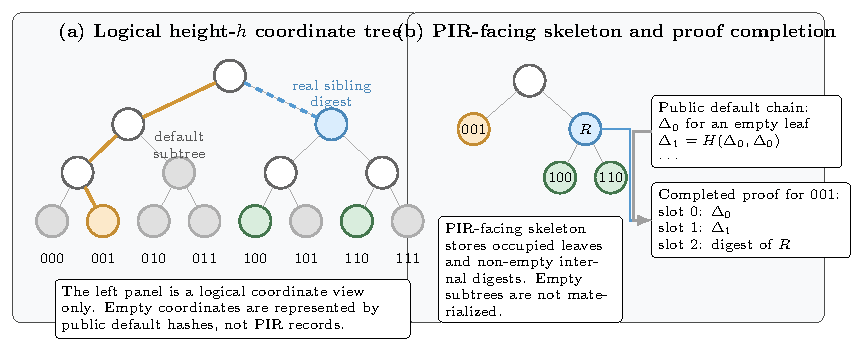
\includegraphics[width=\linewidth]{../figures/sparsetreepir_smt_logical_storage_figure.pdf}
	\caption{Verification and retrieval views of an SMT proof. The verifier checks a standard height-$h$ proof, while the PIR database stores only non-default sibling digests. Empty sibling levels are reconstructed locally from the public default-hash chain.}
	\label{fig:verification-retrieval-view}
\end{figure}

\subsection{From Proof Privacy to Batch PIR}

The privacy goal is query privacy for membership-proof retrieval: given a fixed public SMT snapshot, the server should not learn which occupied leaf the client is proving, nor which authentication path is selected. The tree root, the default-hash chain, and the public retrieval layout may be known to the server.

A simple solution would run one PIR query for every level of the height-$h$ proof. This hides the target, but it treats the proof as $h$ independent lookups and may issue unnecessary queries for levels whose sibling digests are public defaults. Generic batch-PIR schemes can retrieve multiple records privately, but they treat the requested records as an arbitrary batch. They do not specify which SMT proof records should be stored in the PIR database, how default proof entries should be omitted, or how the client should reconstruct the standard SMT proof after retrieval. The sparse setting therefore needs an SMT-specific retrieval layout: simply deleting empty records from a perfect-tree layout is not enough, because the remaining records must still be indexed, partitioned into subdatabases, queried with a fixed query pattern, and mapped back to the correct proof levels.

The construction in this paper stores only non-default sibling digests that may be required by some occupied-leaf membership proof. These records are partitioned into subdatabases so that, for any target, the client needs at most one real record from each subdatabase. The online protocol sends one PIR query to each subdatabase. If the target proof requires a record from that subdatabase, the query selects that record; otherwise, it is a dummy query sampled through the same PIR interface. The server observes a fixed-size batch of well-formed PIR queries, while the client locally determines which responses correspond to proof entries.

\subsection{Retrieval Workload Metrics}

We treat the underlying PIR scheme as a black-box backend. The contribution of the retrieval layout is therefore the database and query profile exposed to existing PIR schemes, rather than a new PIR primitive. For a fixed SMT snapshot, the main quantities are: (i) the number of non-default proof records stored in the PIR database; (ii) the number of PIR subqueries sent for one membership proof; (iii) the maximum subdatabase size; and (iv) the amount of public metadata needed for client-side lookup.

These quantities do not fully determine every PIR implementation's running time, because practical systems differ in packing methods, preprocessing, cryptographic parameters, and query/response formats~\cite{chor,ko97,xpir,sealpir,spiral,simplepir}. They do determine the structural workload given to the backend: sequential execution scales with the queried subdatabases, while parallel execution is often limited by the largest subdatabase. This resource view also clarifies the baseline. Once query privacy is required, the relevant comparison is not ordinary SMT proof serving, but privacy-preserving layouts that store different proof-record sets, issue different numbers of PIR subqueries, and expose different subdatabase sizes.

The resulting design problem is as follows. Given a fixed public SMT snapshot, determine which non-default sibling digests should be stored as PIR records, how these records should be partitioned into subdatabases, and how the client should reconstruct the standard height-$h$ SMT membership proof from PIR responses and public default hashes. Section~\ref{sec:model} formalizes the retrievable record set, the associated target intervals, and the leakage model. Section~\ref{sec:coloring} then presents the SparseTreePIR construction.

\section{Related Work}
\label{sec:related}

\textit{Merkle trees and authenticated data structures.}
Merkle's hash-tree construction~\cite{merkle} underlies authenticated dictionaries and generic authenticated data structures~\cite{padauth,adsgeneric}. Deployed systems use Merkle-style commitments for certificate-transparency logs~\cite{ctv2,ctqueue,crosbywallach}, key-transparency systems~\cite{coniks,transdict,parakeet,optiks}, replicated key-value stores~\cite{dynamo}, append-only authenticated structures~\cite{balloon}, and blockchain or stateless-client commitments~\cite{utreexo,ethereum,zcash}. These systems provide integrity and efficient verification, but they do not hide which proof a client requests. Our setting keeps the SMT snapshot and public metadata visible while hiding the queried occupied leaf.

\textit{Sparse Merkle trees and proof generation.}
SMTs support large logical key spaces by assigning public default hashes to empty subtrees~\cite{sparsemt}. They appear in revocation/transparency maps, authenticated maps, constrained revocation checking, and state-commitment structures such as Jellyfish Merkle Tree~\cite{revtrans,vcer,jmt}. Recent work optimizes proof size, multiproofs, non-membership proofs, batch updates, or alternative authenticated structures~\cite{compactmultiproof,rollupsmt,multicollisiontree}. These systems improve ordinary SMT storage, updates, or proof generation. SparseTreePIR keeps the standard verification interface: the client reconstructs a height-$h$ membership proof. The change is at the retrieval layer, where only non-default sibling digests are queried through PIR and default-empty levels are reconstructed locally.

\textit{Private retrieval of authenticated proofs.}
Private retrieval of authenticated proofs has been studied in multi-client and transparency-log settings~\cite{lueksgoldberg,ctprivacy,kalesct}. The closest structural baseline is TreePIR~\cite{treepir}, which partitions proof nodes of a perfect binary Merkle tree into color classes so that each proof path contains at most one node from each class. SparseTreePIR uses the same one-query-per-color principle, but the database records are different. TreePIR is formulated for a perfect-tree proof layout; an SMT contains public default proof positions that should not be stored or queried through PIR. Pruning those records after expanding to a perfect tree still leaves the wrong query universe. SparseTreePIR instead builds the PIR database directly from non-default sibling digests that can occur in occupied-leaf membership proofs, uses interval metadata for lookup, and reconstructs the ordinary height-$h$ proof with default hashes. Thus it is an SMT proof-retrieval layout, not a new PIR primitive and not a direct TreePIR instantiation.

\textit{Batch PIR and practical PIR backends.}
PIR began with multi-server information-theoretic constructions~\cite{chor} and single-server computational PIR~\cite{ko97,cms}. Batch retrieval uses batch codes and combinatorial batch codes~\cite{batchcodes,cbc}; practical systems use probabilistic batch codes, Cuckoo-style placement, vectorized processing, or constant-weight-code techniques~\cite{sealpir,cuckoo,vectorbatchpir,pirana}. Backends such as XPIR, OnionPIR, Spiral, SimplePIR, PIANO, and YPIR improve communication, server computation, packing, and preprocessing~\cite{xpir,onionpir,spiral,simplepir,piano,ypir}. These systems provide the private-retrieval backend. They do not specify which SMT proof records should enter the PIR database, how to group them into subdatabases, or how to reconstruct the standard SMT proof. SparseTreePIR exposes such a database layout to any compatible backend; real and dummy queries are hidden by the query privacy of the underlying PIR scheme.

\textit{Baselines derived from prior work.}
Existing SMT systems optimize ordinary proof serving: the server traverses the requested coordinate and returns the sibling digests needed for verification~\cite{sparsemt,revtrans,vcer,jmt}. Generic batch-PIR placement can treat the required proof records as an arbitrary batch, yielding PBC-style and unpartitioned active-record baselines. TreePIR applied to a complete SMT gives another baseline, and a height-preserving pruned version can remove public defaults while still keeping the height-$h$ query universe. These are the baselines used in Section~\ref{sec:experiments}. Once query privacy is required, the relevant comparison is between PIR database layouts for the same proof-retrieval task, not against non-private proof serving alone.

\textit{Balancing color subdatabases.}
A valid coloring does not necessarily give an efficient PIR layout: one color subdatabase may be much larger than the others. Perfect-tree coloring reduces the number of queries for perfect Merkle trees, but it does not address the load imbalance caused by sparse SMT snapshots. \ActiveBalance{} is a backend-independent refinement that preserves the same fixed number of PIR queries while reducing the largest queried subdatabase, complementing ordinary SMT proof-generation optimizations.

\section{Problem Formulation and Leakage Model}
\label{sec:model}

This section formalizes the private retrieval problem studied in this paper. We consider a fixed public snapshot of a binary Sparse Merkle Tree (SMT). The tree height, root commitment, occupied-leaf set, public default-hash chain, and the PIR database layout produced during setup are treated as public snapshot information. The privacy goal is query privacy within this fixed snapshot: during online retrieval, the storage server should not learn which occupied leaf is queried, which non-default sibling digests are needed for its proof, or which PIR queries are real rather than dummy queries.

The formal model targets membership-proof retrieval for occupied leaves. Non-membership retrieval over absent coordinates is a natural extension, but it changes the query domain from the public occupied-leaf set to the full logical address space. It also requires metadata for absent coordinate regions and an explicit leakage choice about whether the server learns that the query is a non-membership query. We therefore leave non-membership privacy outside the present model.

A PIR record in this paper means a database record that is retrieved through PIR because it cannot be reconstructed from public default hashes. The record content itself is not assumed to be hidden from the storage server. The protected information is the selected index, or equivalently the queried target leaf, relative to the setup leakage defined below.

\subsection{Fixed-Snapshot Proof Records}

Let $T$ be a fixed binary Sparse Merkle Tree of height $h$, and let $\mathcal{L}$ denote its set of occupied leaves. Hashes are still computed in the standard bottom-up way. The retrieval layout introduced below does not change the SMT hash construction; it only specifies which proof digests are placed in PIR subdatabases. We assume the standard public default-hash chain
\[
\Delta_0,\Delta_1,\ldots,\Delta_{h-1},
\]
where $\Delta_0$ is the default empty-leaf digest and $\Delta_{t+1}=H(\Delta_t\Vert \Delta_t)$ for $0\le t<h-1$. Thus, every empty sibling subtree of height $t$ has publicly reconstructible digest $\Delta_t$.

\begin{definition}[PIR-retrievable sibling node]
For a node $u$ in $T$, let $\operatorname{cnt}(u)$ be the number of occupied leaves in the subtree rooted at $u$. Let $u$ be a non-root node, and let $\operatorname{sib}(u)$ be its sibling. We say that $u$ is a \emph{PIR-retrievable sibling node} if
\[
\operatorname{cnt}(u)>0
\qquad\text{and}\qquad
\operatorname{cnt}(\operatorname{sib}(u))>0.
\]
The set of all PIR-retrievable sibling nodes is denoted by $\mathcal{A}(T)$.
\end{definition}

The first condition ensures that $u$ itself has a non-default digest. The second condition ensures that $u$ can appear as a sibling node in the membership proof of at least one occupied target leaf. Thus $\mathcal{A}(T)$ contains exactly the non-default sibling digests that may have to be retrieved through PIR. Empty sibling subtrees remain outside the PIR database because their digests are publicly reconstructible from the default-hash chain.
We sometimes call nodes in $\mathcal{A}(T)$ \emph{active proof nodes}; this is only shorthand for PIR-retrievable non-default sibling nodes, not for arbitrary non-empty SMT nodes.

\begin{proposition}[Minimal non-default PIR record set]
\label{prop:active-record-minimality}
Fix a public height-$h$ SMT snapshot $T$ and the public default-hash chain, and assume the SMT hash function is collision resistant. In the record-based retrieval model where a PIR record supplies one proof sibling digest and public default values are filled locally, $\mathcal{A}(T)$ is exactly the set of non-default sibling digests that may be required by some occupied-leaf membership proof, except with negligible hash-collision probability. Consequently, any PIR database that supports all occupied-leaf membership proofs must make one digest for every node in $\mathcal{A}(T)$ retrievable, while no default-empty sibling position needs a PIR record.
\end{proposition}

\begin{proof}
If $u\in\mathcal{A}(T)$, then $u$ is non-empty and $\operatorname{sib}(u)$ is also non-empty. Choose any occupied leaf in the subtree of $\operatorname{sib}(u)$; the standard membership proof for that leaf contains the digest of $u$ as a sibling digest. By collision resistance, a non-empty subtree digest is computationally distinct from the corresponding public default digest except with negligible probability. Thus a record-based private retrieval layout that reconstructs every occupied-leaf proof must make this digest retrievable. Conversely, if a proof sibling subtree is empty, its digest is the public value $\Delta_t$ for the corresponding height $t$ and is reconstructed locally. A non-empty node whose sibling subtree is empty is not a sibling for any occupied target leaf. Therefore the necessary and sufficient non-default PIR record set is precisely $\mathcal{A}(T)$.
\end{proof}

\begin{definition}[PIR-retrievable sibling set]
For any occupied leaf $\ell \in \mathcal{L}$, let
\[
\mathsf{Path}(\ell)\subseteq \mathcal{A}(T)
\]
denote the sequence of all PIR-retrievable sibling nodes in the standard Merkle proof of $\ell$, ordered from higher to lower proof levels.
\end{definition}

Equivalently, $\mathsf{Path}(\ell)$ contains exactly those sibling nodes on the standard height-$h$ proof of $\ell$ whose subtrees contain at least one occupied leaf. Sibling levels whose subtrees are empty are not PIR records and are later filled locally with the corresponding default hash.

Although the full SMT proof length is always $h$, the number of PIR records in $\mathsf{Path}(\ell)$ may be smaller than $h$, because some levels correspond only to publicly reconstructible default-empty nodes.

Let
\[
m=\max_{\ell\in\mathcal{L}} |\mathsf{Path}(\ell)|
\]
be the \emph{retrieval width} of the snapshot, namely the maximum number of non-default sibling digests that can appear in one occupied-leaf membership proof. Equivalently, this is the active width used by SparseTreePIR. By construction, $m\le h$. Once the PIR-retrievable record set is fixed, this same quantity is also the number of color classes and the batch width of the one-query-per-color retrieval layout. Throughout the paper, $[m]$ denotes $\{1,\ldots,m\}$.

The case $|\mathcal{L}|=1$ is degenerate: no occupied target has a non-default sibling subtree, so $\mathcal{A}(T)=\emptyset$, $m=0$, and no PIR query is issued. Unless explicitly stated otherwise, the rest of the paper assumes $|\mathcal{L}|\ge 2$.

The role of $m$ is analogous to the role of $h$ in TreePIR only after public default-empty levels have been removed from the PIR database layout. It is not a tunable parameter chosen by the balancing algorithm; it is a public resource parameter of the fixed SMT snapshot. The verifier still receives a height-$h$ proof after client-side reconstruction. The retrieval width only measures how many proof positions may require private retrieval under the record-based retrieval model.

\begin{remark}[Why $m$ can be much smaller than $h$]
The value of $m$ is necessarily instance-dependent because it depends on where the occupied leaves branch. The setup phase publishes $m$ as part of the public layout, just as a perfect-tree TreePIR setup publishes height $h$. To interpret this parameter, suppose $n$ occupied leaves are sampled uniformly from a logical universe of size $U=2^h$, and condition on one target leaf. At proof level $t$ above the leaf, the sibling subtree contains $2^t$ logical leaves, so the probability that this level contributes a non-default sibling digest is
\[
1-\frac{\binom{U-1-2^t}{n-1}}{\binom{U-1}{n-1}}
\approx 1-\exp\!\left(-\frac{(n-1)2^t}{U-1}\right).
\]
Thus the expected number of PIR-retrievable proof positions for a random target is the sum of these probabilities over $t=0,\ldots,h-1$. When $n\ll U$, most low levels have empty sibling subtrees and only the levels near the branching depth of the occupied set contribute; the retrieval width therefore tracks the branching structure of the occupied leaves rather than the logical height. In adversarial layouts, the sharp worst-case bound remains $m\le\min\{h,n-1\}$.
\end{remark}

This paper focuses on target-private retrieval of \emph{membership} proofs for occupied leaves in a fixed public SMT snapshot. This scope matches the proof-retrieval setting in which the client privately asks for the authentication material of an existing committed object. Non-membership retrieval is a natural extension, but it changes the object being hidden. The target domain becomes the full logical coordinate space rather than the public occupied-leaf set; a proof may certify an empty coordinate, a divergence from the nearest occupied prefix, or a gap between existing keys; and the protocol must specify whether the server should learn that the query is for an absent coordinate. Consequently, the interval metadata would have to range over logical coordinates or absent-coordinate regions, not only over occupied-leaf ranks. We therefore keep non-membership SparseTreePIR outside the present formal model and treat it as a separate extension requiring its own metadata and leakage model.

\subsection{Target-Rank Intervals}

To support efficient indexing, we associate each PIR-retrievable sibling node with the interval of target leaves for which it acts as a proof sibling. This is not the subtree interval of $u$ itself. Order the occupied leaves by their logical SMT positions and let $r(\ell)\in\{0,\ldots,|\mathcal{L}|-1\}$ be the occupied-leaf rank of $\ell$. Let $s=\operatorname{sib}(u)$, and define the \emph{target-rank interval}
\[
I_{\mathsf{srv}}(u) = [L(s),R(s)]
\]
as the interval of occupied-leaf ranks covered by the sibling subtree of $u$. Thus $L(s)$ and $R(s)$ are rank endpoints, not heap-index endpoints in the full logical coordinate space. Then, for any occupied leaf $\ell$,
\[
u \in \mathsf{Path}(\ell) \Longleftrightarrow r(\ell) \in I_{\mathsf{srv}}(u).
\]

Since every binary subtree corresponds to a contiguous interval in leaf order, the resulting target-rank intervals form a laminar family: any two intervals are either disjoint, or one contains the other. This structure underlies both the coloring method and the indexing method.
The intervals are public lookup metadata derived from the fixed snapshot and the public occupied-leaf order. Publishing them is therefore part of the setup leakage below; it does not attempt to hide the occupancy pattern or density of the snapshot. If the occupied-leaf set itself were sensitive, the layout would need additional occupancy-hiding mechanisms, such as dummy occupied leaves or oblivious metadata publication, which are outside the present query-privacy model.

\begin{figure}[!t]
\centering
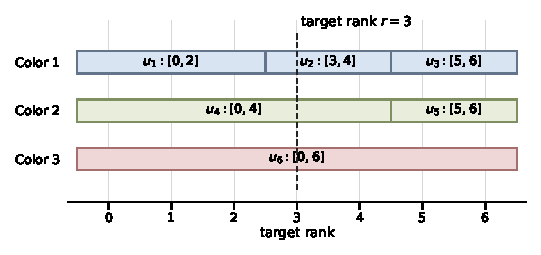
\includegraphics[width=\linewidth]{../figures/sparsetreepir_interval_coloring_figure.pdf}
\caption{Target-rank intervals and proper coloring. Each non-default sibling digest is associated with the target ranks whose proofs require it. Intervals form a laminar family, and a proper coloring ensures that any vertical target rank intersects at most one record from each color subdatabase.}
\label{fig:interval-coloring}
\end{figure}

\subsection{Coloring and Load Metrics}

The constructions below use $m$ color classes, where $m$ is the retrieval width defined above. Since $m\le h$, the resulting batch profile is no wider than the SMT verifier height. Section~\ref{sec:correctness} later states the corresponding model-specific lower-bound argument: under the one-query-per-color model, a proof requiring $m$ PIR records needs $m$ distinct colors.

\begin{definition}[Proper coloring]
A map
\[
\varphi:\mathcal{A}(T)\rightarrow[m]
\]
is a \emph{proper coloring} if for every occupied leaf $\ell\in\mathcal{L}$ and every two distinct nodes $u,v\in\mathsf{Path}(\ell)$, we have
\[
u\neq v \Longrightarrow \varphi(u)\neq \varphi(v).
\]
\end{definition}

A proper coloring ensures that every membership proof needs at most one real PIR record from each color subdatabase.

For a color $c\in[m]$, let
\[
\mathcal{D}_c=\{u\in\mathcal{A}(T): \varphi(u)=c\}
\]
be the corresponding color subdatabase, with size $N_c=|\mathcal{D}_c|$. Let $N=|\mathcal{A}(T)|$, and let
\[
\overline{N}=N/m
\]
be the average subdatabase size. The main optimization target in this paper is to keep the color subdatabases as balanced as possible while preserving proper coloring. In particular, we track
\[
M(\varphi)=\max_c N_c,
\qquad
\Delta_N(\varphi)=\max_c N_c-\min_c N_c,
\]
and the normalized maximum-subdatabase ratio
\[
R(\varphi)=\frac{M(\varphi)}{\overline{N}}.
\]
Here $M(\varphi)$ is the direct structural bottleneck, while $\Delta_N(\varphi)$ and $R(\varphi)$ indicate how far the partition is from an equal split.

The \ActiveBalance{} scheme is self-contained. It first constructs a feasible coloring by a first-fit traversal of the laminar interval forest, and then refines that coloring by subtree-level color permutations that directly improve the global subdatabase loads.

\begin{definition}[Client-side inputs and public metadata]
For a target leaf $\ell$, the client uses the following local inputs and public metadata before issuing PIR queries:
\begin{enumerate}[leftmargin=2em]
  \item the tree height $h$ and the position of $\ell$ in the SMT;
  \item the default-hash chain $\Delta_0,\ldots,\Delta_{h-1}$;
  \item the occupied-leaf rank $r(\ell)$ of the target within the public ordered set of occupied leaves;
  \item for each color $c\in[m]$, a public metadata table
  \[
  \mathcal{M}_c=\bigl((I_{\mathsf{srv}}(u),\delta(u))\bigr)_{u\in\mathcal{D}_c},
  \]
  sorted by interval, where the two endpoints of $I_{\mathsf{srv}}(u)$ are occupied-leaf ranks and $\delta(u)=h-\operatorname{depth}(u)$ denotes the proof level of $u$ measured from leaf to root.
\end{enumerate}
\end{definition}

The PIR subdatabases store node digests. The level and interval information required for client-side proof reconstruction is carried by the public metadata tables rather than by PIR records.

\subsection{Setup Leakage and Target Privacy}

The retrieval protocol in this paper hides the queried target leaf inside one \emph{fixed public SMT instance}; it does not aim to hide the entire occupancy pattern of that instance. We model the storage server's snapshot-level view with the following deterministic setup leakage.

We assume the underlying backend is a correct single-item PIR scheme with query privacy over each fixed subdatabase: for any two valid indices in the same subdatabase, the server-observable query distributions are computationally indistinguishable. We also require the real and dummy queries for a given subdatabase to use the same PIR query interface and the same observable query/response lengths. Otherwise, a backend-level length or format difference could reveal whether a color is real or dummy.

\begin{definition}[Setup leakage]
\label{def:leakagefunction}
Let setup on a fixed SMT snapshot $T$ produce retrieval width $m$, PIR-retrievable node set $\mathcal{A}(T)$, coloring $\varphi:\mathcal{A}(T)\to[m]$, color subdatabases $\{\mathcal{D}_c\}_{c=1}^{m}$, and public metadata tables $\{\mathcal{M}_c\}_{c=1}^{m}$. Let $N_c=|\mathcal{D}_c|$. The setup leakage visible to the storage server is
\[
\begin{aligned}
\mathcal{L}_{\mathsf{setup}}(T)=
\Bigl(&h,\mathsf{root}(T),\mathcal{L},
\{\Delta_t\}_{t=0}^{h-1},\\
&\mathcal{A}(T),m,\varphi,
\{(\mathcal{D}_c,\mathcal{M}_c,N_c)\}_{c=1}^{m}
\Bigr).
\end{aligned}
\]
Thus the leakage includes the fixed occupancy pattern, the committed root, the public default-hash chain, the PIR-retrievable node set, the coloring, the color subdatabases, the public metadata, and the subdatabase sizes. For an online target $\ell$, it does not include $\ell$, the set $\mathsf{Path}(\ell)$ of required PIR records, the set of colors containing real proof records, or the selected item index inside any color subdatabase. The only target-independent online shape revealed by the protocol is that every retrieval sends exactly one PIR subquery to each of the $m$ color subdatabases.
\end{definition}

The hidden query information consists of the target leaf $\ell$, equivalently the required PIR record set $\mathsf{Path}(\ell)$, as well as which color positions correspond to real retrievals rather than dummy subqueries and which item index is privately selected inside each color subdatabase.

\begin{table}[t]
\centering
\caption{Server-visible setup state and hidden query information}
\label{tab:leakage}
\scriptsize
\setlength{\tabcolsep}{4pt}
\begin{tabular}{>{\raggedright\arraybackslash}p{0.45\linewidth}>{\raggedright\arraybackslash}p{0.45\linewidth}}
\toprule
Visible to the storage server & Hidden by PIR queries \\
\midrule
root, occupied-leaf set, default-hash chain, PIR-retrievable node set, color subdatabases, interval metadata, color assignment, subdatabase sizes, retrieval width $m$
&
target leaf $\ell$, required PIR records, which color slots are real or dummy, selected item index inside each color subdatabase \\
\bottomrule
\end{tabular}
\end{table}

We make this leakage profile explicit. The retrieval layout is precomputed once for a fixed SMT snapshot and is treated as server-visible structure thereafter. Our privacy claim is therefore \emph{query privacy relative to a server-visible PIR database layout}, rather than structure privacy for the whole sparse tree. The corresponding transcript view has a fixed query shape: the server sees one well-formed PIR query per color, while the real/dummy roles are client-local.

The privacy model is honest-but-curious with respect to the storage server. A malicious server cannot make an incorrect digest verify against the public SMT root except with the usual hash-collision probability, but it can cause retrieval failure or equivocate about published metadata unless the subdatabases and metadata are authenticated. Such authenticated publication, for example by committing to the public layout or by using an authenticated PIR service layer, is complementary to the query-privacy mechanism studied here.

\begin{definition}[Target privacy game]
\label{def:privacygame}
Let $\mathcal{L}_{\mathsf{setup}}(T)$ be the setup leakage in Definition~\ref{def:leakagefunction}. In the experiment $\mathsf{PrivTarget}_{\mathcal{A}}(\lambda)$, the challenger runs setup for the fixed SMT snapshot and gives $\mathcal{L}_{\mathsf{setup}}(T)$ to the adversary $\mathcal{A}$. The adversary chooses two occupied target leaves $\ell_0,\ell_1\in\mathcal{L}$. The challenger samples $b\leftarrow\{0,1\}$, runs the batch query-generation algorithm for $\ell_b$, and gives the full batch query transcript to $\mathcal{A}$. The adversary outputs a bit $b'$. Its advantage is
\[
\operatorname{Adv}^{\mathsf{target}}_{\mathcal{A}}
=\left|\Pr[b'=b]-\frac12\right|.
\]
The protocol is target-private relative to $\mathcal{L}_{\mathsf{setup}}(T)$ if this advantage is negligible for every efficient adversary.
\end{definition}

\begin{definition}[Dummy query distribution]
\label{def:dummyquery}
For a non-empty color subdatabase $\mathcal{D}_c$ of size $N_c$, a dummy query samples an index $d_c\leftarrow \{0,\ldots,N_c-1\}$ independently of the target leaf and invokes the same query algorithm $\mathsf{PIR.Query}(\mathcal{D}_c,d_c)$ used for real records.
\end{definition}

For dummy positions, the client uses Definition~\ref{def:dummyquery} and discards the response locally. The setup layout exposes only non-empty color subdatabases. Implementations that allow empty color classes can remove them during setup or pad them with one public dummy record.

\section{SparseTreePIR Construction}
\label{sec:coloring}

This section gives the fixed-snapshot retrieval protocol. Offline preprocessing constructs color subdatabases from the compressed non-default SMT representation; online retrieval sends one target-independent batch of PIR queries and reconstructs the standard height-$h$ proof with public default hashes. Figure~\ref{fig:workflow} summarizes the setup and retrieval flow.

\begin{figure}[H]
	\centering
	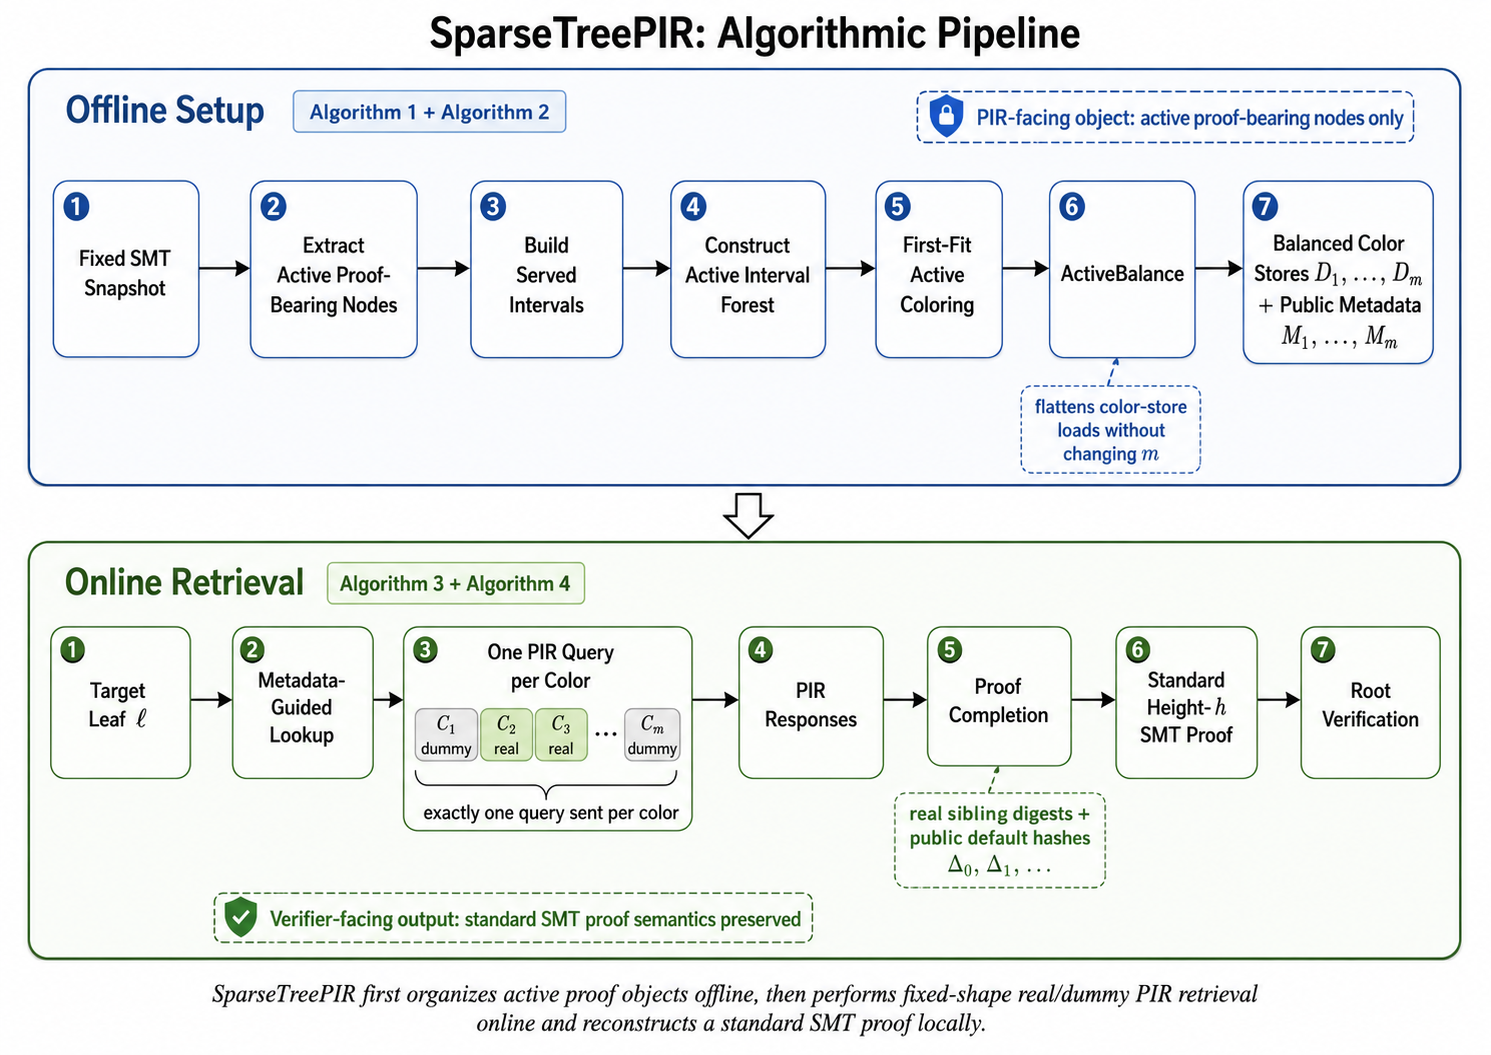
\includegraphics[width=\linewidth]{../figures/sparsetreepir_algorithmic_pipeline.png}
	\caption{SparseTreePIR pipeline. Setup builds color subdatabases and public metadata; online retrieval sends one PIR query per color and reconstructs the standard SMT proof with public default hashes.}
	\label{fig:workflow}
\end{figure}

\subsection{Offline Preprocessing}

Offline setup is run once for a fixed public SMT snapshot. It identifies the non-default sibling digests that may appear in membership proofs, records for each digest its target-rank interval and proof level, builds the laminar interval forest, colors it, and publishes the resulting subdatabases and metadata. The procedure never materializes the full logical coordinate tree.

The first-fit stage is a feasibility step: it traverses the interval forest and assigns every node the smallest color not used on its strict ancestor chain. \ActiveBalance{} then applies legal subtree recolorings to reduce the lexicographically sorted load vector $\operatorname{sort}_{\downarrow}(|\mathcal{D}_1|,\ldots,|\mathcal{D}_m|)$ while preserving the coloring constraint. Once setup has built the color subdatabases and metadata tables, online retrieval needs only interval lookup, one PIR query per color, and the public default-hash chain.

\subsection{\ActiveBalance{}: Load Balancing by Subtree Recoloring}

A valid coloring guarantees that each proof needs at most one real record from each color subdatabase, but it does not guarantee balanced subdatabase sizes. \ActiveBalance{} preserves the retrieval width $m$ and changes only the assignment of records to colors. For a rooted subtree $U$ of the interval forest, any permutation of colors not used by strict ancestors of $U$ can be applied uniformly inside $U$ without violating the coloring constraint. \ActiveBalance{} evaluates such candidate recolorings and accepts a move only if it decreases the lexicographic load vector
\[
\Psi(\varphi)=
\operatorname{sort}_{\downarrow}(N_1,\ldots,N_m),
\]
where $N_c=|\mathcal{D}_c|$. The accepted-move rule reduces the largest subdatabase first and then flattens the remaining count vector. Section~\ref{sec:correctness} gives the preservation argument, balance certificate, and runtime bound.


\subsection{Target-Independent Online Query Generation}

After preprocessing, the client uses only public metadata to determine which color subdatabases contain proof records for the target. For each color $c$, the metadata table $\mathcal{M}_c$ is sorted by target-rank interval. Since intervals with the same color are disjoint, one binary search returns either a unique matching record or no matching record.

\begin{algorithm}[H]
\caption{Online query generation: one PIR subquery per color}
\label{alg:query}
\begin{algorithmic}[1]
\Require Target leaf $\ell$ with occupied-leaf rank $r(\ell)$, color subdatabases $\{\mathcal{D}_c\}_{c=1}^{m}$, public metadata tables $\{\mathcal{M}_c\}_{c=1}^{m}$, underlying PIR query generator $\mathsf{PIR.Query}$
\Ensure Batch query $\mathcal{Q}=\{Q_c\}_{c=1}^{m}$ and client-side selection map $\{\tau_c\}_{c=1}^{m}$
\State Initialize $\mathcal{Q}\gets\emptyset$
\For{$c=1$ \textbf{to} $m$}
  \State Perform a binary search for $r(\ell)$ in the target-rank interval projection of $\mathcal{M}_c$
  \If{there exists exactly one interval containing $r(\ell)$}
    \State Let $j_c$ be the position of that node in $\mathcal{D}_c$
    \State Set $\tau_c\gets j_c$ and $Q_c\gets\mathsf{PIR.Query}(\mathcal{D}_c,j_c)$
  \Else
    \State Set $\tau_c\gets \bot$ and sample $d_c\leftarrow\{0,\ldots,|\mathcal{D}_c|-1\}$
    \State Set $Q_c\gets\mathsf{PIR.Query}(\mathcal{D}_c,d_c)$
  \EndIf
  \State Add $Q_c$ to $\mathcal{Q}$
\EndFor
\State Send $\mathcal{Q}$ to the server and keep $\{\tau_c\}$ locally
\State \Return $\mathcal{Q},\{\tau_c\}_{c=1}^{m}$
\end{algorithmic}
\end{algorithm}
\vspace{-0.5em}

\subsection{Client-Side Proof Reconstruction}

The server returns one PIR response for each color subdatabase. The client decodes all responses, keeps only those marked in the selection map, initializes the proof array with public default hashes, and overwrites the levels indicated by the metadata with the retrieved non-default digests. The result is a complete height-$h$ SMT membership proof, not a compressed proof, and can be verified by the standard bottom-up Merkle procedure. Thus SparseTreePIR changes the retrieval layout, not the verifier's proof format.

\section{Correctness, Privacy, and Complexity}
\label{sec:correctness}

This section states the main guarantees used by the construction and evaluation. Detailed proof steps are standard consequences of laminar interval structure, PIR query privacy, and default-hash SMT verification. As in Section~\ref{sec:model}, let $N=|\mathcal{A}(T)|$ and $n=|\mathcal{L}|$; for $n=1$, no non-default sibling digest is needed and no PIR query is issued.

\begin{theorem}[Tightness of $m$ in one-query-per-color retrieval]
\label{thm:mincolor}
For a fixed height-$h$ SMT snapshot with $n\ge2$ occupied leaves, let
\[
    m=\max_{\ell\in\mathcal{L}}|\mathsf{Path}(\ell)|.
\]
Then $m$ colors are necessary and sufficient in the one-query-per-color retrieval model. A proper $m$-coloring can be computed in $O(N)$ time once the interval forest has been constructed. Moreover,
\[
m\le \min\{h,n-1\},
\]
and this bound is tight for every $h$ and $n\ge 2$.
\end{theorem}

\noindent\emph{Proof sketch.}
Necessity follows from any target proof containing $m$ active proof nodes: all such nodes must receive distinct colors. For sufficiency, the target-rank intervals form a laminar family, and two records co-occur in one proof exactly when their intervals contain the same target rank. Coloring by depth in the interval forest is therefore proper and uses exactly the maximum number of intervals covering any rank, namely $m$. The upper bound follows because one proof has at most one non-default sibling per SMT level and its non-empty sibling subtrees are disjoint, each containing an occupied leaf different from the target. Tightness is witnessed by placing leaves so that a fixed target has a non-empty sibling subtree at each of $k=\min\{h,n-1\}$ distinct depths.

\begin{remark}
Theorem~\ref{thm:mincolor} is where the SMT formulation departs from a naive complete-tree view. A full-tree or height-preserving pruned layout is pinned to the proof height $h$, whereas SparseTreePIR is governed by the maximum number of non-default sibling positions on any occupied-leaf proof.
\end{remark}

\begin{theorem}[Correctness of retrieval and proof reconstruction]
\label{thm:correctness}
Assume the underlying single-item PIR backend is correct. Under any proper coloring, Algorithm~\ref{alg:query} recovers exactly the non-default sibling digests needed by the target proof using exactly $m$ PIR subqueries. After filling all other proof levels with public default hashes, the client obtains a standard height-$h$ SMT membership proof.
\end{theorem}

\noindent\emph{Proof sketch.}
Proper coloring ensures that each color subdatabase contains at most one real proof record for any target. Hence the client either queries that unique record or sends a dummy query in the same subdatabase. Correct PIR responses return all non-default sibling digests, and every omitted proof level corresponds to an empty sibling subtree whose digest is the public default value $\Delta_t$.

\begin{theorem}[Target privacy under setup leakage]
\label{prop:privacy}
Assume the setup leakage profile and target-privacy game of Definition~\ref{def:privacygame}. Assume $m$ is polynomially bounded in the security parameter, as holds when $h$ is polynomially bounded. If each underlying PIR query is query-private over its color subdatabase and dummy queries are sampled as in Definition~\ref{def:dummyquery}, then SparseTreePIR is target-private relative to $\mathcal{L}_{\mathsf{setup}}(T)$.
\end{theorem}

\noindent\emph{Proof sketch.}
Conditioned on setup leakage, the server already knows the snapshot, subdatabases, metadata, sizes, and the fact that every retrieval sends one query per color. The only target-dependent values are the selected PIR indices and the real/dummy labels. For each color, PIR query privacy hides the selected index, and a dummy query is distributed as a well-formed query over the same subdatabase. A standard hybrid over the polynomially many colors makes the complete batch transcripts for any two occupied targets computationally indistinguishable.

\begin{theorem}[Structural lower bound for color-subdatabase balance]
\label{thm:structlb}
Let $N=|\mathcal{A}(T)|$ and let $m$ be the number of colors. For a node $v$ in the interval forest, let $d(v)$ be the number of active proof nodes on the path from the root of its connected component to $v$, including $v$, and let $\operatorname{desc}(v)$ be the number of strict descendants of $v$. Define
\[
B(T)=
\max\left\{
\left\lceil \frac{N}{m}\right\rceil,\,
\max_{v:\ d(v)<m}
\left\lceil \frac{\operatorname{desc}(v)}{m-d(v)}\right\rceil
\right\}.
\]
If the second maximum is over an empty set, it is omitted.
Then every proper coloring $\varphi:\mathcal{A}(T)\rightarrow[m]$ satisfies
\[
\max_{c\in[m]} |\mathcal{D}_c| \ge B(T).
\]
\end{theorem}

\noindent\emph{Proof sketch.}
The first term is the equal-split lower bound. For the second term, the $d(v)$ nodes on the root-to-$v$ interval-forest path must use distinct colors, and every strict descendant of $v$ co-occurs with each of them. The descendants can therefore use only $m-d(v)$ remaining colors, so one such color receives at least the stated pigeonhole count.

\begin{proposition}[ActiveBalance certificate and complexity]
\label{prop:activebalancecert}
Let $\varphi_{\mathsf{out}}$ be the coloring returned by \ActiveBalance{}, and let
\[
U=\max_{c\in[m]}|\mathcal{D}_c(\varphi_{\mathsf{out}})|.
\]
Let $\operatorname{OPT}$ be the smallest possible value of $\max_c|\mathcal{D}_c|$ over all proper $m$-colorings. Then
\[
\frac{U}{\operatorname{OPT}}\le \frac{U}{B(T)}.
\]
Thus $U/B(T)$ is an a posteriori balance certificate for the returned coloring. The procedure accepts only finitely many improving moves and, if not stopped by a round limit, returns a local optimum under the allowed subtree-permutation moves. With at most $R_1$ passes, its implementation runs in $O(R_1Nm^3)$ time and uses $O(Nm)$ additional space.
\end{proposition}

\noindent\emph{Proof sketch.}
The certificate follows from Theorem~\ref{thm:structlb}: $\operatorname{OPT}\ge B(T)$. Termination follows because each accepted move strictly decreases the sorted load vector over a finite set of colorings. In one pass, subtree histograms take $O(Nm)$ space, and each of the $N$ candidate roots solves an assignment problem of size at most $m$, giving $O(Nm^3)$ time per pass.

\begin{theorem}[End-to-end SparseTreePIR guarantee]
\label{thm:endtoend}
Fix a public height-$h$ SMT snapshot $T$ with active proof-node set $\mathcal{A}(T)$, number of colors $m$, a proper coloring $\varphi$, color subdatabases $\mathcal{D}_1,\ldots,\mathcal{D}_m$, and public metadata tables $\mathcal{M}_1,\ldots,\mathcal{M}_m$. Assume that the underlying single-item PIR backend is correct and query-private for each subdatabase, and that dummy queries are generated as in Definition~\ref{def:dummyquery}. Then SparseTreePIR satisfies the following end-to-end guarantee for every occupied target leaf:
\begin{enumerate}[leftmargin=2em]
  \item the client reconstructs a valid standard height-$h$ SMT membership proof;
  \item the retrieval is target-private relative to the setup leakage in Definition~\ref{def:leakagefunction} and the target-privacy game in Definition~\ref{def:privacygame};
  \item the PIR database contains exactly $N=|\mathcal{A}(T)|$ digest records, and the public metadata size is $O(N)$;
  \item client-side lookup and proof completion together cost $O(m\log N+h)$ time;
  \item the PIR-backend workload is determined by the load vector $(|\mathcal{D}_1|,\ldots,|\mathcal{D}_m|)$: a sequential execution performs one PIR query over each color subdatabase, while a parallel execution is bottlenecked by the largest per-color backend call.
\end{enumerate}
\end{theorem}

\noindent\emph{Proof sketch.}
Correctness follows from Theorem~\ref{thm:correctness}; privacy follows from Theorem~\ref{prop:privacy}. The construction stores one digest per active proof record and constant-size metadata per record. Query indexing is one binary search per color, giving $O(m\log N)$ time, and proof reconstruction scans $h$ levels. Finally, Algorithm~\ref{alg:query} issues one PIR call to each color subdatabase, so backend cost composes over the subdatabase sizes.


\section{Experimental Evaluation}
\label{sec:experiments}

This section evaluates SparseTreePIR as a PIR-based retrieval layout for fixed-snapshot SMT membership proofs. Direct SMT proof serving is only a functional reference, because a direct request reveals the target coordinate and authentication path. The relevant comparison is therefore between privacy-preserving layouts that expose different database sizes, query patterns, and subdatabase sizes to the same PIR backends.

\subsection{Experimental Setup}

We use six SMT key sets: five account-key snapshots derived from public Polygon zkEVM and ZKsync Era RPC data, and one FuelLabs SMT test-vector workload. Each key set is mapped into height-$128$ and height-$256$ coordinate spaces, with duplicate coordinates merged. These are reproducible account-key snapshots rather than full archival state-tree dumps.

We ran all backend measurements on a workstation with a 13th Gen Intel Core i5-13500HX CPU, 20 hardware threads, and 15 GiB RAM in an Ubuntu 22.04.5 environment. For each height-$128$ workload, we sampled $50$ occupied targets under each of three target-sampling seeds and recorded averages. Online communication counts the total upload and download bytes of the measured PIR calls. Timing columns report backend preprocessing, query generation, and response generation only; they exclude one-time layout construction, public metadata publication, and local proof reconstruction. The artifact records the extraction scripts, command lines, environment record, and raw CSV outputs.

\subsection{Privacy-Preserving Layouts}

We compare SparseTreePIR with four privacy-preserving layouts. Complete-tree TreePIR treats the SMT as a full height-$h$ tree. Height-preserving pruned TreePIR removes public default records from the searched payloads but still sends one query per proof level, so its width remains $h$. PBC-style SMT is an optimistic generic batch-placement baseline over the same active proof records, using three replicated copies and $\lceil1.5m\rceil$ balanced buckets. Unpartitioned active-record PIR stores each active proof record once but searches one global active-record database for each proof slot.

\begin{table*}[!t]
\centering
\caption{Height-$128$ workload profiles and induced costs for privacy-preserving retrieval layouts. Height-$256$ has the same active records and SparseTreePIR width for these key sets; the verifier-side proof still has length $256$.}
\label{tab:real_workload_shape}
\scriptsize
\setlength{\tabcolsep}{4pt}
\begin{tabular}{lrrrrrrr}
\toprule
Workload & Keys & PIR rec. & Subq. $m$ & Pruned q/max & PBC b/max & Unpart. max & STPIR max \\
\midrule
FuelLabs SMT vectors & 100   & 198   & 9  & 128 / 40   & 14 / 43   & 198   & 23 \\
Polygon recent       & 384   & 766   & 11 & 128 / 168  & 17 / 136  & 766   & 70 \\
ZKsync sample        & 956   & 1910  & 13 & 128 / 370  & 20 / 287  & 1910  & 147 \\
Polygon multi-window & 1348  & 2694  & 14 & 128 / 530  & 21 / 385  & 2694  & 193 \\
Polygon broad        & 7040  & 14078 & 17 & 128 / 2762 & 26 / 1625 & 14078 & 829 \\
ZKsync broad         & 7740  & 15478 & 17 & 128 / 3014 & 26 / 1786 & 15478 & 911 \\
\bottomrule
\end{tabular}
\end{table*}

Table~\ref{tab:real_workload_shape} shows that SparseTreePIR uses only $9$--$17$ subqueries, whereas height-preserving pruned TreePIR still issues $128$ queries at height $128$ and $256$ queries at height $256$. For the broad ZKsync workload, $15478$ active proof records are partitioned into $17$ subdatabases, and the largest SparseTreePIR subdatabase contains $911$ records; the Pruned TreePIR-$128$ baseline has a largest subdatabase of $3014$ records.

\begin{figure}[!t]
\centering
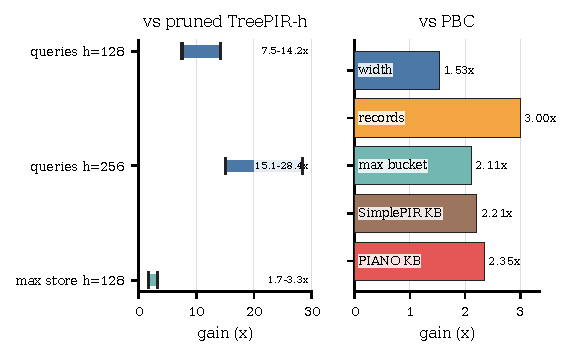
\includegraphics[width=\linewidth]{../figures/sparsetreepir_gain_summary_bars.pdf}
\caption{Summary of layout and backend gains. SparseTreePIR reduces query width and maximum searched subdatabase size at the layout level, and these improvements translate into lower online communication with SimplePIR and PIANO.}
\label{fig:gain_summary}
\end{figure}

Figure~\ref{fig:gain_summary} separates the main sources of improvement. SparseTreePIR stores only non-default proof records, replaces the height-$h$ pruned TreePIR query pattern with $m$ subqueries, and balances per-color subdatabases. Complete-tree TreePIR is much larger still: at height $128$ and $256$, full coordinate-tree layouts are more than \(4.3{\cdot}10^{34}\times\) and \(10^{73}\times\) larger than the largest active-record layout. \ActiveBalance{} reaches the structural lower bound $B(T)$ on five of the six height-$128$ workloads, is within $1.045\times$ on the FuelLabs workload, and reduces the maximum subdatabase size by $10.8\%$--$21.6\%$ relative to a node-local greedy initializer.

\subsection{Experiments with Existing PIR Backends}

We next evaluate whether the structural improvements translate to existing PIR implementations. The SimplePIR experiment uses the official Go API~\cite{simplepir} for setup, query generation, response generation, and recovery over the induced subdatabases, and checks that the recovered digest records match the requested proof records. This is our main end-to-end backend experiment. The PIANO experiment uses the public PIANO artifact~\cite{piano} with the same subdatabase-size vectors, and serves as a secondary implementation-based check of the layout-induced backend workload.

\begin{table}[!t]
\centering
\caption{Repeated implementation-based backend results on real height-$128$ workloads. Each entry is a baseline/SparseTreePIR cost ratio averaged over six workloads, three seeds, and $50$ requested occupied targets per seed. Server-response gain is SimplePIR response-generation time; preprocessing gain is backend preprocessing only and excludes layout construction and metadata publication.}
\label{tab:real_backend_summary}
\scriptsize
\setlength{\tabcolsep}{3pt}
\resizebox{\linewidth}{!}{%
\begin{tabular}{lrrrrrrr}
\toprule
Backend & Runs & Query-count gain & Max-size gain & Comm. gain & Client-query gain & Server-response gain & Preproc. gain \\
\midrule
SimplePIR full API & $3\times50$ & $1.5\times$ & -- & $2.1\times$ & $1.7\times$ & $1.8\times$ & $2.3\times$ \\
PIANO local runner & $3\times50$ & $1.5\times$ & $1.9\times$ & $2.3\times$ & $2.4\times$ & -- & $3.1\times$ \\
\bottomrule
\end{tabular}
\par}
\end{table}

Table~\ref{tab:real_backend_summary} is the main backend result. Against the PBC-style SMT baseline, SparseTreePIR gives $2.1\times$ lower online communication under SimplePIR and $2.3\times$ lower online communication under PIANO. Under SimplePIR, server response-generation time is $1.8\times$ lower on average. PIANO answer-time measurements are not reported because the artifact's small-database counters are often zero or quantized. Client query generation and backend preprocessing also improve, with gains ranging from $1.7\times$ to $3.1\times$. These gains are not caused by changing the PIR primitive: both schemes are measured through the same backend in each row. They come from the database layout exposed to the backend: the PBC-style baseline stores three copies over approximately $1.5m$ buckets, whereas SparseTreePIR stores one copy over $m$ subdatabases.

\subsection{Reproducibility and Scope}

All tables in this section are generated by repository scripts from checked-in workload summaries and backend outputs. Raw per-workload SimplePIR and PIANO measurements, seed-level summaries, environment records, and command lines are included in the artifact. The protocol scope is fixed-snapshot membership-proof retrieval for occupied leaves; non-membership retrieval and dynamic updates require additional metadata, leakage choices, and amortization analysis.

\section{Conclusion and Future Directions}
\label{sec:conclusion}

This paper presented SparseTreePIR, a retrieval layout for target-private membership proofs in fixed binary Sparse Merkle Tree snapshots. SparseTreePIR keeps the standard height-$h$ SMT proof interface unchanged: the verifier receives one sibling digest per level, while the PIR backend stores and retrieves only the non-default sibling digests that cannot be derived from the public default-hash chain. Public interval metadata identifies which proof records are relevant to a target leaf, and a target-independent batch query with real and dummy PIR queries hides the requested authentication path. The client reconstructs the standard SMT proof locally by combining retrieved digests with public default hashes.

Our analysis shows that private proof retrieval is governed by the non-default proof records in the occupied-leaf skeleton, rather than by the full logical height of the SMT. In the one-query-per-subdatabase model, the batch width is the maximum number of non-default sibling digests on any occupied-leaf proof path. SparseTreePIR also addresses load balancing across PIR subdatabases: \ActiveBalance{} reduces the maximum subdatabase size by applying subtree-level permutations of subdatabase labels while preserving the same batch query pattern. On six SMT-derived workloads, the resulting batch width is only 9--17 for height-128 and height-256 proofs, and the layout reduces both the number of subqueries and the largest searched subdatabase relative to pruned TreePIR-style, generic batch-placement, and flat single-database baselines. SimplePIR and PIANO experiments further show lower online communication than the PBC-style SMT baseline without changing the underlying PIR schemes.

Future work should extend the retrieval model to non-membership proofs, dynamic SMT updates, and deployed sparse authenticated stores such as revocation-transparency maps and Jellyfish Merkle Tree-style state stores~\cite{revtrans,jmt}. These settings require additional leakage choices, update and rebuilding policies, and end-to-end engineering analysis for metadata publication, record packing, preprocessing, and backend selection. A complementary theoretical direction is to strengthen the current instance-specific load-balance certificate into an a priori approximation guarantee for broader interval-based proof workloads.

\begin{thebibliography}{99}

\bibitem{merkle}
R. C. Merkle,
\newblock ``A Certified Digital Signature,''
\newblock in \emph{Advances in Cryptology---CRYPTO '89 Proceedings}, G. Brassard, Ed., LNCS 435, Springer, 1990, pp. 218--238.

\bibitem{ctv2}
B. Laurie, E. Messeri, and R. Stradling,
\newblock ``Certificate Transparency Version 2.0,''
\newblock RFC 9162, Internet Engineering Task Force, Dec. 2021.

\bibitem{ctqueue}
B. Laurie,
\newblock ``Certificate Transparency,''
\newblock \emph{ACM Queue}, vol. 12, no. 8, pp. 10--19, 2014.

\bibitem{crosbywallach}
S. A. Crosby and D. S. Wallach,
\newblock ``Efficient Data Structures for Tamper-Evident Logging,''
\newblock in \emph{Proc. 18th USENIX Security Symposium (USENIX Security)}, 2009.

\bibitem{dynamo}
G. DeCandia, D. Hastorun, M. Jampani, G. Kakulapati, A. Lakshman, A. Pilchin, S. Sivasubramanian, P. Vosshall, and W. Vogels,
\newblock ``Dynamo: Amazon's Highly Available Key-Value Store,''
\newblock in \emph{Proc. 21st ACM Symp. Operating Systems Principles (SOSP)}, 2007, pp. 205--220.

\bibitem{padauth}
A. Anagnostopoulos, M. T. Goodrich, and R. Tamassia,
\newblock ``Persistent Authenticated Dictionaries and Their Applications,''
\newblock in \emph{Information Security}, LNCS 2200, Springer, 2001, pp. 379--393.

\bibitem{coniks}
M. S. Melara, A. Blankstein, J. Bonneau, E. W. Felten, and M. J. Freedman,
\newblock ``CONIKS: Bringing Key Transparency to End Users,''
\newblock in \emph{Proc. 24th USENIX Security Symposium (USENIX Security)}, 2015, pp. 383--398.

\bibitem{transdict}
I. Tzialla, A. Kothapalli, B. Parno, and S. Setty,
\newblock ``Transparency Dictionaries with Succinct Proofs of Correct Operation,''
\newblock in \emph{Proc. Network and Distributed System Security Symposium (NDSS)}, 2022.

\bibitem{parakeet}
H. Malvai, L. Kokoris-Kogias, A. Sonnino, E. Ghosh, E. Ozturk, K. Lewi, and S. F. Lawlor,
\newblock ``Parakeet: Practical Key Transparency for End-to-End Encrypted Messaging,''
\newblock in \emph{Proc. Network and Distributed System Security Symposium (NDSS)}, 2023.

\bibitem{optiks}
J. Len, M. Chase, E. Ghosh, K. Laine, and R. Cruz Moreno,
\newblock ``OPTIKS: An Optimized Key Transparency System,''
\newblock in \emph{Proc. 33rd USENIX Security Symposium (USENIX Security)}, 2024, pp. 4355--4372.

\bibitem{revtrans}
B. Laurie and E. Kasper,
\newblock ``Revocation Transparency,''
\newblock Google Research technical report, Sep. 2012.

\bibitem{vcer}
D. Koisser, P. Jauernig, G. Tsudik, and A.-R. Sadeghi,
\newblock ``V'CER: Efficient Certificate Validation in Constrained Networks,''
\newblock in \emph{Proc. 31st USENIX Security Symposium (USENIX Security)}, 2022, pp. 4491--4508.

\bibitem{utreexo}
B. Bailey and S. Sankagiri,
\newblock ``Merkle Trees Optimized for Stateless Clients in Bitcoin,''
\newblock in \emph{Financial Cryptography and Data Security}, LNCS 12676, Springer, 2021, pp. 451--466.

\bibitem{ethereum}
G. Wood,
\newblock ``Ethereum: A Secure Decentralised Generalised Transaction Ledger,''
\newblock Ethereum Project Yellow Paper, 2014.

\bibitem{zcash}
D. E. Hopwood, S. Bowe, T. Hornby, and N. Wilcox,
\newblock ``Zcash Protocol Specification,''
\newblock Version 2023.4.0, 2023.

\bibitem{sparsemt}
R. Dahlberg, T. Pulls, and R. Peeters,
\newblock ``Efficient Sparse Merkle Trees: Caching Strategies and Secure (Non-)Membership Proofs,''
\newblock \emph{Cryptology ePrint Archive}, Paper 2016/683, 2016.

\bibitem{jmt}
Z. Gao, Y. Hu, and Q. Wu,
\newblock ``Jellyfish Merkle Tree,''
\newblock Diem Association technical paper, revised Jan. 12, 2021.

\bibitem{compactmultiproof}
L. Ramabaja and A. Avdullahu,
\newblock ``Compact Merkle Multiproofs,''
\newblock arXiv preprint arXiv:2002.07648, 2020.

\bibitem{rollupsmt}
B. Ma, V. N. Pathak, L. Liu, and S. Ruj,
\newblock ``One-Phase Batch Update on Sparse Merkle Trees for Rollups,''
\newblock arXiv preprint arXiv:2310.13328, 2023.

\bibitem{zksyncdataset}
M. I. Silva, J. Messias, and B. Livshits,
\newblock ``A Public Dataset For the ZKsync Rollup,''
\newblock arXiv preprint arXiv:2407.18699, 2024.

\bibitem{multicollisiontree}
M. Petkus,
\newblock ``Efficient (Non-)Membership Tree from Multicollision-Resistance with Applications to Zero-Knowledge Proofs,''
\newblock Cryptology ePrint Archive, Paper 2024/1259, 2024.

\bibitem{treepir}
Q. Cao, S. H. Dau, R. Gagiano, D. Huynh, X. Yi, P. L. Le, Q.-H. Luu, E. Viterbo, Y.-C. Huang, J. Zhu, M. M. Jalalzai, and C. Feng,
\newblock ``TreePIR: Efficient Private Retrieval of Merkle Proofs via Tree Colorings with Fast Indexing and Zero Storage Overhead,''
\newblock in \emph{Proc. IEEE Symp. Security and Privacy (SP)}, 2025, pp. 4476--4494.

\bibitem{ctprivacy}
S. Eskandarian, E. Messeri, J. Bonneau, and D. Boneh,
\newblock ``Certificate Transparency with Privacy,''
\newblock \emph{Proc. Privacy Enhancing Technologies}, vol. 2017, no. 4, pp. 329--344, 2017.

\bibitem{kalesct}
D. Kales, O. Omolola, and S. Ramacher,
\newblock ``Revisiting User Privacy for Certificate Transparency,''
\newblock in \emph{Proc. IEEE European Symp. Security and Privacy (EuroS\&P)}, 2019, pp. 432--447.

\bibitem{lueksgoldberg}
W. Lueks and I. Goldberg,
\newblock ``Sublinear Scaling for Multi-Client Private Information Retrieval,''
\newblock in \emph{Financial Cryptography and Data Security}, LNCS 8975, Springer, 2015, pp. 168--186.

\bibitem{chor}
B. Chor, O. Goldreich, E. Kushilevitz, and M. Sudan,
\newblock ``Private information retrieval,''
\newblock \emph{Journal of the ACM}, vol. 45, no. 6, pp. 965--981, 1998.

\bibitem{ko97}
E. Kushilevitz and R. Ostrovsky,
\newblock ``Replication Is Not Needed: Single Database, Computationally-Private Information Retrieval,''
\newblock in \emph{Proc. 38th Annu. IEEE Symp. Foundations of Computer Science (FOCS)}, 1997, pp. 364--373.

\bibitem{cms}
C. Cachin, S. Micali, and M. Stadler,
\newblock ``Computationally Private Information Retrieval with Polylogarithmic Communication,''
\newblock in \emph{Advances in Cryptology---EUROCRYPT '99}, LNCS 1592, Springer, 1999, pp. 402--414.

\bibitem{batchcodes}
Y. Ishai, E. Kushilevitz, R. Ostrovsky, and A. Sahai,
\newblock ``Batch Codes and Their Applications,''
\newblock in \emph{Proc. 36th Annu. ACM Symp. Theory of Computing (STOC)}, 2004, pp. 262--271.

\bibitem{cbc}
D. R. Stinson, R. Wei, and M. B. Paterson,
\newblock ``Combinatorial Batch Codes,''
\newblock \emph{Advances in Mathematics of Communications}, vol. 3, no. 1, pp. 13--27, 2009.

\bibitem{cuckoo}
R. Pagh and F. F. Rodler,
\newblock ``Cuckoo Hashing,''
\newblock \emph{Journal of Algorithms}, vol. 51, no. 2, pp. 122--144, 2004.

\bibitem{xpir}
C. Aguilar-Melchor, J. Barrier, L. Fousse, and M.-O. Killijian,
\newblock ``XPIR: Private Information Retrieval for Everyone,''
\newblock \emph{Proc. Priv. Enhancing Technol.}, vol. 2016, no. 2, pp. 155--174, 2016.

\bibitem{sealpir}
S. Angel, H. Chen, K. Laine, and S. Setty,
\newblock ``PIR with Compressed Queries and Amortized Query Processing,''
\newblock in \emph{Proc. IEEE Symp. Security and Privacy (SP)}, 2018, pp. 962--979.

\bibitem{onionpir}
M. H. Mughees, H. Chen, and L. Ren,
\newblock ``OnionPIR: Response Efficient Single-Server PIR,''
\newblock in \emph{Proc. ACM SIGSAC Conference on Computer and Communications Security (CCS)}, 2021, pp. 2292--2306.

\bibitem{spiral}
S. J. Menon and D. J. Wu,
\newblock ``Spiral: Fast, High-Rate Single-Server PIR via FHE Composition,''
\newblock in \emph{Proc. IEEE Symp. Security and Privacy (SP)}, 2022, pp. 930--947.

\bibitem{simplepir}
A. Henzinger, M. M. Hong, H. Corrigan-Gibbs, S. Meiklejohn, and V. Vaikuntanathan,
\newblock ``One Server for the Price of Two: Simple and Fast Single-Server Private Information Retrieval,''
\newblock in \emph{Proc. 32nd USENIX Security Symposium (USENIX Security)}, 2023, pp. 3889--3905.

\bibitem{piano}
M. Zhou, A. Park, W. Zheng, and E. Shi,
\newblock ``Piano: Extremely Simple, Single-Server PIR with Sublinear Server Computation,''
\newblock in \emph{Proc. IEEE Symp. Security and Privacy (SP)}, 2024, pp. 4296--4314.

\bibitem{ypir}
S. J. Menon and D. J. Wu,
\newblock ``YPIR: High-Throughput Single-Server PIR with Silent Preprocessing,''
\newblock in \emph{Proc. 33rd USENIX Security Symposium (USENIX Security)}, 2024, pp. 5985--6002.

\bibitem{vectorbatchpir}
M. H. Mughees and L. Ren,
\newblock ``Vectorized Batch Private Information Retrieval,''
\newblock in \emph{Proc. IEEE Symp. Security and Privacy (SP)}, 2023, pp. 437--452.

\bibitem{pirana}
J. Liu, J. Li, D. Wu, and K. Ren,
\newblock ``PIRANA: Faster Multi-query PIR via Constant-weight Codes,''
\newblock in \emph{Proc. IEEE Symp. Security and Privacy (SP)}, 2024, pp. 4315--4330.

\bibitem{adsgeneric}
A. Miller, M. Hicks, J. Katz, and E. Shi,
\newblock ``Authenticated Data Structures, Generically,''
\newblock in \emph{Proc. 41st ACM SIGPLAN-SIGACT Symposium on Principles of Programming Languages (POPL)}, 2014, pp. 411--423.

\bibitem{balloon}
T. Pulls and R. Peeters,
\newblock ``Balloon: A Forward-Secure Append-Only Persistent Authenticated Data Structure,''
\newblock in \emph{Computer Security---ESORICS 2015}, LNCS 9326, Springer, 2015, pp. 622--641.

\end{thebibliography}

\appendices

\section{Supplementary Algorithms and Proof Details}
\label{app:proofs}

This appendix gives pseudocode and proof details omitted from the main text. They are included for auditability; the main correctness, privacy, and complexity claims are stated in Section~\ref{sec:correctness}.

\setcounter{algorithm}{0}
\renewcommand{\thealgorithm}{A.\arabic{algorithm}}

\begin{algorithm}[H]
\caption{Offline preprocessing}
\label{alg:app_setup}
\footnotesize
\begin{algorithmic}[1]
\Require Fixed SMT snapshot \(T\), occupied leaf set \(\mathcal{L}\), balancing passes \(R_1\)
\Ensure Retrieval width \(m\), color subdatabases \(\{\mathcal{D}_c\}_{c=1}^{m}\), metadata tables \(\{\mathcal{M}_c\}_{c=1}^{m}\), coloring \(\varphi\)
\State Traverse the compressed non-default SMT representation and compute occupied-leaf counts and rank endpoints.
\For{each non-root node \(u\)}
    \If{\(\operatorname{cnt}(u)>0\) and \(\operatorname{cnt}(\operatorname{sib}(u))>0\)}
        \State Add \(u\) to \(\mathcal{A}(T)\).
        \State Record its digest, proof level \(\delta(u)\), and target-rank interval \(I_{\mathsf{srv}}(u)\).
    \EndIf
\EndFor
\State Build the laminar interval forest from the target-rank intervals.
\State Set \(m\gets \max_{\ell\in\mathcal{L}}|\mathsf{Path}(\ell)|\).
\State Compute an initial proper coloring \(\varphi:\mathcal{A}(T)\rightarrow[m]\).
\State Apply \(\ActiveBalance{}\) to refine \(\varphi\) for at most \(R_1\) passes.
\For{each color \(c\in[m]\)}
    \State Build \(\mathcal{D}_c\) from digest records with color \(c\).
    \State Build \(\mathcal{M}_c\) from \((I_{\mathsf{srv}}(u),\delta(u),\operatorname{pos}_c(u))\), sorted by interval.
\EndFor
\State \Return \(m,\{\mathcal{D}_c\},\{\mathcal{M}_c\},\varphi\)
\end{algorithmic}
\end{algorithm}

\begin{algorithm}[H]
\caption{\ActiveBalance{} by subtree recoloring}
\label{alg:app_activebalance}
\footnotesize
\begin{algorithmic}[1]
\Require Interval forest \(F\), proper coloring \(\varphi\), colors \([m]\), pass limit \(R_1\)
\Ensure Refined proper coloring \(\varphi\)
\For{\(r=1,\ldots,R_1\)}
    \State \(\mathsf{changed}\gets\mathsf{false}\); compute the current load vector \((|\mathcal{D}_1|,\ldots,|\mathcal{D}_m|)\).
    \For{each subtree root \(v\) of \(F\)}
        \State \(C_{\mathrm{anc}}\gets\{\varphi(a):a\text{ is a strict ancestor of }v\}\)
        \State \(C_{\mathrm{avail}}\gets [m]\setminus C_{\mathrm{anc}}\)
        \State Build the cost matrix induced by recoloring the subtree of \(v\) with colors in \(C_{\mathrm{avail}}\).
        \State Solve the resulting assignment problem to obtain the best subtree color permutation \(\pi_v\).
        \If{applying \(\pi_v\) strictly decreases the lexicographically sorted load vector}
            \State Recolor the subtree of \(v\), update the loads, and set \(\mathsf{changed}\gets\mathsf{true}\).
        \EndIf
    \EndFor
    \If{\(\mathsf{changed}=\mathsf{false}\)}
        \State \textbf{break}
    \EndIf
\EndFor
\State \Return \(\varphi\)
\end{algorithmic}
\end{algorithm}

\subsection{Record and Width Bounds}

\emph{Minimal record set.}
For every node \(u\in\mathcal{A}(T)\), both \(u\) and its sibling contain occupied leaves. Choosing any occupied target leaf under \(\operatorname{sib}(u)\), the standard SMT membership proof for that target contains the digest of \(u\). Since \(u\) is non-empty, collision resistance implies that its digest is computationally distinct from the public default digest for the same subtree height, except with negligible probability. Thus a record-based retrieval database that supports all occupied-leaf membership proofs must make this digest retrievable. Conversely, if a sibling subtree is empty, its digest is the public default value \(\Delta_t\), and if a non-empty node has an empty sibling, it is not a proof sibling for any occupied target. Hence \(\mathcal{A}(T)\) is the necessary and sufficient non-default PIR record set.

\emph{Number of records.}
Every active proof node has a parent whose two SMT children are both non-empty. Conversely, each such branching parent contributes at most its two child roots to \(\mathcal{A}(T)\). The compressed non-default skeleton induced by \(n\) occupied leaves has at most \(n-1\) branching internal nodes, so \(|\mathcal{A}(T)|\le 2(n-1)\). Equality is reached by full binary occupied-leaf skeletons in which both children of every branching node correspond to non-empty SMT subtrees.

\emph{Tightness of retrieval width.}
The necessity and sufficiency of \(m\) colors follow from the interval-forest argument in Theorem~\ref{thm:mincolor}. To realize the bound, let \(k=\min\{h,n-1\}\), choose the target coordinate \(0^h\), and add occupied leaves \(0^d1\,0^{h-d-1}\) for \(d=0,\ldots,k-1\). These leaves make \(k\) distinct sibling subtrees on the target path non-empty, so the target proof contains \(k\) retrievable non-default siblings.

\subsection{Correctness and Privacy}

For a proper coloring, same-color target-rank intervals are disjoint. Otherwise, one occupied target rank would lie in two same-color intervals, and the corresponding proof would contain two records of the same color, contradicting properness. Therefore Algorithm~\ref{alg:query} has at most one real record per color. Correctness of the underlying PIR backend returns all selected real records, while public default hashes fill every empty proof level. This produces the standard height-\(h\) proof array used by ordinary SMT verification.

For target privacy, condition on \(\mathcal{L}_{\mathsf{setup}}(T)\). The server already knows the snapshot, subdatabases, metadata, sizes, and the fact that one query is sent to each color. For one color, replacing the query generated for target \(\ell_0\) by the query generated for target \(\ell_1\) changes only the hidden PIR index or changes a real query into a well-formed dummy query over the same subdatabase. PIR query privacy makes the replacement computationally indistinguishable. A hybrid over the polynomially bounded number of colors gives the batch transcript indistinguishability claimed in Theorem~\ref{prop:privacy}.

\subsection{ActiveBalance and Runtime}

A subtree recoloring is valid because all colors used by strict ancestors of the subtree are removed from the available-color set. Pairs inside the subtree remain distinct under a common permutation; pairs outside the subtree do not change; and any co-occurring inside/outside pair must involve a strict ancestor whose color is unavailable inside the subtree. Thus the recoloring preserves properness.

The balance certificate follows from Theorem~\ref{thm:structlb}: since every valid coloring has maximum subdatabase size at least \(B(T)\), a returned layout with maximum size \(U\) satisfies \(U/\mathrm{OPT}\le U/B(T)\). Termination follows because every accepted move strictly decreases the sorted load vector over finitely many colorings. For complexity, one pass computes subtree color histograms in \(O(Nm)\) space and evaluates \(N\) assignment problems of size at most \(m\), giving \(O(Nm^3)\) time per pass and \(O(R_1Nm^3)\) over \(R_1\) passes.

Metadata construction costs \(O(N\log N)\) time to sort the per-color interval tables and \(O(N)\) space. Online lookup performs one binary search per color, for \(O(m\log N)\) time, and client-side proof reconstruction scans the height-\(h\) proof array, for \(O(h)\) additional time and space.

\section{Additional Experimental Tables}
\label{app:experiments}

\begin{table}[H]
\centering
\caption{\ActiveBalance{} ablation on real height-\(128\) workloads.}
\label{tab:app_activebalance}
\scriptsize
\setlength{\tabcolsep}{3pt}
\resizebox{\linewidth}{!}{%
\begin{tabular}{lrrrrrrr}
\toprule
Workload & PIR rec. & \(m\) & Lower & Greedy max & AB max & Red. & Meta KB \\
\midrule
FuelLabs SMT vectors & 198   & 9  & 22  & 26   & 23  & 11.5\% & 4.6 \\
Polygon recent       & 766   & 11 & 70  & 83   & 70  & 15.7\% & 18.0 \\
ZKsync sample        & 1910  & 13 & 147 & 180  & 147 & 18.3\% & 44.8 \\
Polygon multi-window & 2694  & 14 & 193 & 236  & 193 & 18.2\% & 63.1 \\
Polygon broad        & 14078 & 17 & 829 & 929  & 829 & 10.8\% & 330.0 \\
ZKsync broad         & 15478 & 17 & 911 & 1162 & 911 & 21.6\% & 362.8 \\
\bottomrule
\end{tabular}
\par}
\end{table}

\begin{table}[H]
\centering
\caption{Raw SimplePIR full-API means behind Table~\ref{tab:real_backend_summary}. Communication is KB per requested proof; timings are milliseconds.}
\label{tab:app_simplepir_raw}
\scriptsize
\setlength{\tabcolsep}{3pt}
\resizebox{\linewidth}{!}{%
\begin{tabular}{lrrrrrr}
\toprule
Workload & PBC KB & Sparse KB & PBC query & Sparse query & PBC answer & Sparse answer \\
\midrule
Fuel vectors         & 12.000 & 5.906  & 9.061  & 5.936  & 0.033 & 0.023 \\
Polygon recent       & 25.500 & 11.688 & 12.180 & 7.609  & 0.044 & 0.029 \\
ZKsync sample        & 43.125 & 20.719 & 15.817 & 9.684  & 0.076 & 0.038 \\
Polygon multi-window & 51.844 & 25.375 & 17.792 & 10.633 & 0.081 & 0.047 \\
Polygon broad        & 133.250& 62.156 & 32.367 & 17.223 & 0.245 & 0.114 \\
ZKsync broad         & 138.938& 65.344 & 32.302 & 17.679 & 0.268 & 0.120 \\
\bottomrule
\end{tabular}
\par}
\end{table}

\begin{table}[H]
\centering
\caption{Per-workload implementation-based backend gains against the PBC-style SMT baseline. Entries are baseline/SparseTreePIR ratios averaged over three target-sampling seeds.}
\label{tab:app_backend_workloads}
\scriptsize
\setlength{\tabcolsep}{3pt}
\resizebox{\linewidth}{!}{%
\begin{tabular}{lrrrrrr}
\toprule
Workload & Query count & SimplePIR comm. & SimplePIR query & PIANO comm. & PIANO query & PIANO max \\
\midrule
FuelLabs SMT vectors & 14 / 9  & \(2.0\times\) & \(1.5\times\) & \(3.2\times\) & \(3.4\times\) & \(1.9\times\) \\
Polygon recent       & 17 / 11 & \(2.2\times\) & \(1.6\times\) & \(3.1\times\) & \(2.7\times\) & \(1.9\times\) \\
ZKsync sample        & 20 / 13 & \(2.1\times\) & \(1.6\times\) & \(2.1\times\) & \(1.8\times\) & \(2.0\times\) \\
Polygon multi-window & 21 / 14 & \(2.0\times\) & \(1.7\times\) & \(2.1\times\) & \(2.1\times\) & \(2.0\times\) \\
Polygon broad        & 26 / 17 & \(2.1\times\) & \(1.9\times\) & \(2.1\times\) & \(3.1\times\) & \(2.0\times\) \\
ZKsync broad         & 26 / 17 & \(2.1\times\) & \(1.8\times\) & \(2.1\times\) & \(2.1\times\) & \(2.0\times\) \\
\bottomrule
\end{tabular}
\par}
\end{table}

\noindent\textbf{Artifact contents.}
The repository includes workload extraction scripts, checked-in workload summaries, raw per-seed backend outputs, aggregate mean and standard-deviation CSVs, and the environment record used for the measurements in Section~\ref{sec:experiments}.
